% Name: Minimum spanning tree
% Description: A weighted graph with its minimum spanning tree in green: six edges of total weight 39.
% Tags: minimum spanning tree, Kruskal, Prim, weighted graph

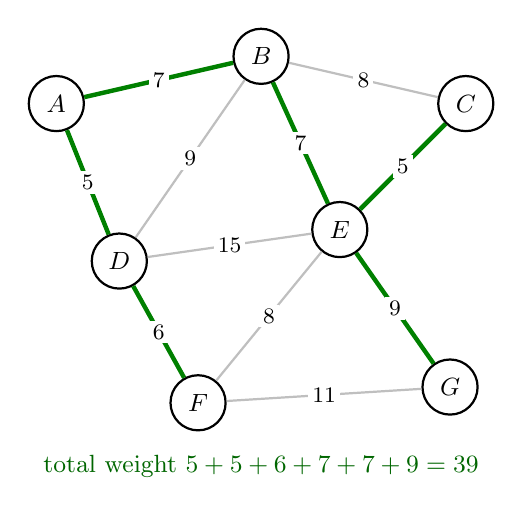
\begin{tikzpicture}[
  vertex/.style={circle, draw, thick, fill=white, minimum size=7mm, inner sep=0pt, font=\small},
  weight/.style={font=\footnotesize, fill=white, inner sep=1.5pt},
  mst/.style={line width=1.6pt, green!50!black},
]
  \node[vertex] (A) at (0,3) {$A$};
  \node[vertex] (B) at (2.6,3.6) {$B$};
  \node[vertex] (C) at (5.2,3) {$C$};
  \node[vertex] (D) at (0.8,1) {$D$};
  \node[vertex] (E) at (3.6,1.4) {$E$};
  \node[vertex] (F) at (1.8,-0.8) {$F$};
  \node[vertex] (G) at (5,-0.6) {$G$};
  % Kruskal takes AD 5, CE 5, DF 6, AB 7, BE 7, and EG 9, and skips the rest.
  \foreach \u/\v in {B/C, B/D, D/E, E/F, F/G}
    \draw[thick, gray!50] (\u) -- (\v);
  \foreach \u/\v in {A/B, A/D, C/E, D/F, B/E, E/G}
    \draw[mst] (\u) -- (\v);
  \foreach \u/\v/\w in {A/B/7, A/D/5, B/C/8, B/D/9, B/E/7, C/E/5, D/E/15, D/F/6, E/F/8, E/G/9, F/G/11}
    \path (\u) -- node[weight] {\w} (\v);
  \node[font=\small, green!40!black] at (2.6,-1.6) {total weight $5+5+6+7+7+9 = 39$};
\end{tikzpicture}
